\begin{example}~
\label{ex:multiple_channels}
	Let the set of confidential information be represented as $P = \set{(1,3),(2,1),(3,4),(4,1),(5,5),(6,9)}$. Assume that \AgentOne sends this information encrypted as $Q = \set{(1,12),(2,1),(3,16),(4,1),(5,17),(6,18)}$. To avoid detection, \AgentOne sends part of the information on three different channels such that $Q_1 = \set{(1,12),(2,1)}$, $Q_2 = \set{(3,16),(4,1)}$ and $Q_3 = \set{(5,17),(6,18)}$. \newline 

	We define the relations $P$, $Q_1$, $Q_2$, and $Q_3$ in \relview\ as follows: \newline

	\begin{figure}[ht]
		\centering
		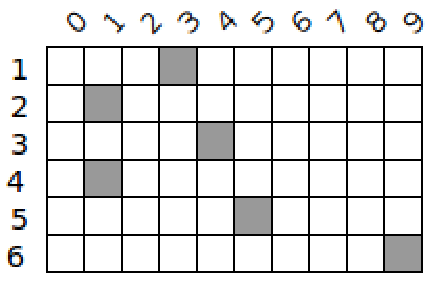
\includegraphics[scale=0.65]{Figures/PDF/Relview/P.pdf}
		\caption{Relation $P$ for Example~\ref{ex:multiple_channels}.}
		\label{fig:multiple_channels_p}
	\end{figure}

	\begin{figure}[ht]
		\centering
		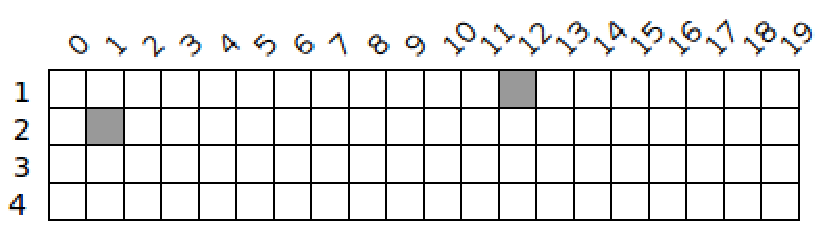
\includegraphics[scale=0.65]{Figures/PDF/Relview/QQ1.pdf}
		\caption{Relation $Q_1$ for Example~\ref{ex:multiple_channels}.}
		\label{fig:multiple_channels_q1}
	\end{figure}
	
	\begin{figure}[ht]
		\centering
		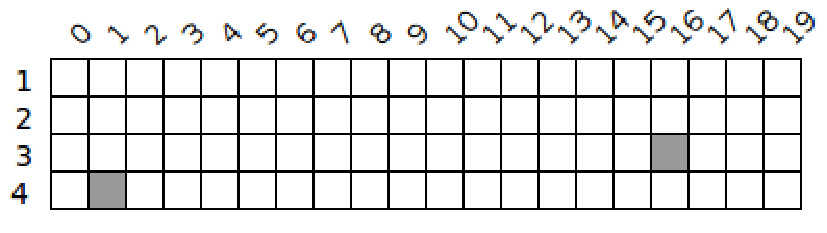
\includegraphics[scale=0.65]{Figures/PDF/Relview/QQ2.pdf}
		\caption{Relation $Q_2$ for Example~\ref{ex:multiple_channels}.}
		\label{fig:multiple_channels_q2}
	\end{figure}
	
	\begin{figure}[ht]
		\centering
		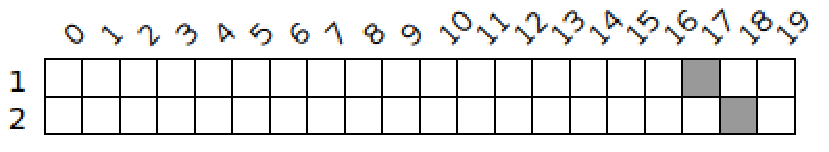
\includegraphics[scale=0.65]{Figures/PDF/Relview/QQ3.pdf}
		\caption{Relation $Q_3$ for Example~\ref{ex:multiple_channels}.}
		\label{fig:multiple_channels_q3}
	\end{figure}

 	Suppose that the analyst has programmed the monitor of the communication channels to combine the information that has been sent on the channels corresponding to with the union operation ( $\!\!\!\STjoin\!\!\!$ ) and the relational sum operation ($+$). The relation generated by the combination of the three channels is as follows: \newline

	\begin{figure}[ht]
		\centering
		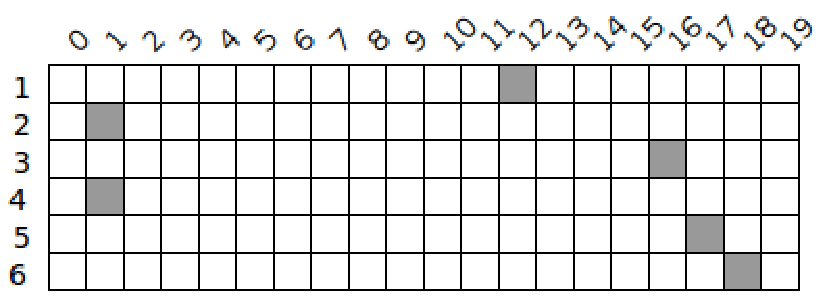
\includegraphics[scale=0.65]{Figures/PDF/Relview/Q.pdf}
		\caption{Relation $(Q_1 \STjoin Q_2) + Q_3$ for Example~\ref{ex:multiple_channels}.}
		\label{fig:multiple_channels_q}
	\end{figure}

	We verify the existence of an abstraction relation by executing Program~\ref{prog:test} ($Result = Test(P, (Q_1 \STjoin Q_2) + Q_3)$). \newline

	\begin{figure}[ht]
		\centering
		
\includegraphics[scale=0.65]{Figures/PDF/Relview/True.pdf}
		\caption{Relation $Result$ for Example~\ref{ex:multiple_channels}.}
		\label{fig:multiple_channels_result}
	\end{figure}

	Therefore, the test has passed so we can compute the abstraction relation by executing Program~\ref{prog:compute} ($X = Compute(P,(Q_1 \STjoin Q_2) + Q_3,R)$) where $R$ is the filtering relation. \newline

	\begin{figure}[ht]
		\centering
		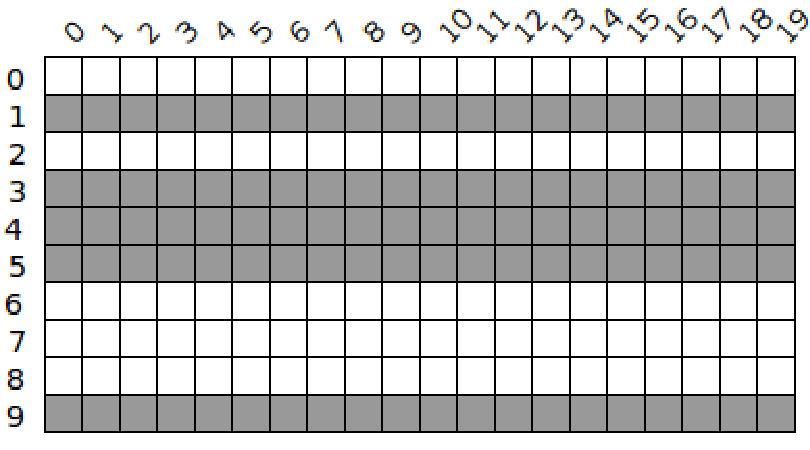
\includegraphics[scale=0.65]{Figures/PDF/Relview/R.pdf}
		\caption{Filtering relation $R$ for Example~\ref{ex:multiple_channels}.}
		\label{fig:multiple_channels_r}
	\end{figure}

	\begin{figure}[ht]
		\centering
		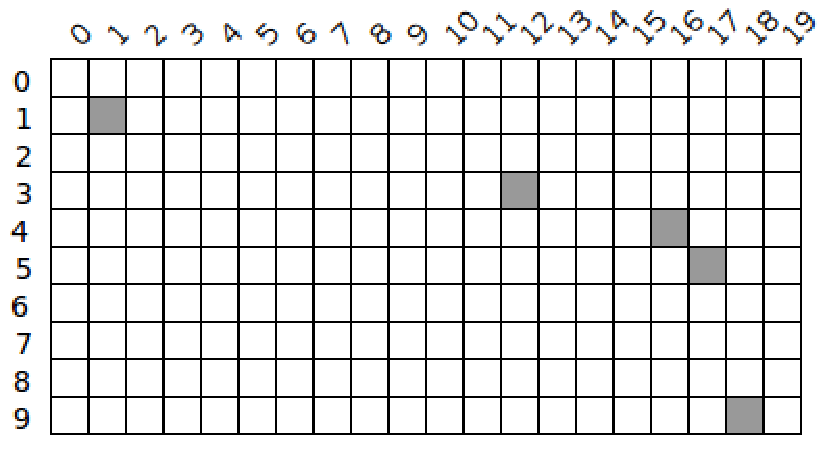
\includegraphics[scale=0.65]{Figures/PDF/Relview/XR.pdf}
		\caption{Abstraction relation $X$ for Example~\ref{ex:multiple_channels}.}
		\label{fig:multiple_channels_x}
	\end{figure}
	
	\newpage 
\end{example}